\chapter[Tool demonstration: Molten Salt Breeder Reactor]{SaltProc 
demonstration: Molten Salt Breeder Reactor}

This chapter describes the fuel cycle analysis of the \gls{MSBR} obtained 
using the open-source python package, SaltProc. The development was initially 
started as a part of my master thesis \cite{rykhlevskii_advanced_2018} in 
2017.  In this effort, for verification purpose, I assumed ideal extraction 
efficiency (e.g., 100\% of target isotope mass extracted) because all 
available in the literature results also rely on this assumption.

The main results presented in this chapter have been published in: A. 
Rykhlevskii, J.W. Bae, and K. D. Huff, ``Modeling and simulation of online 
reprocessing in the thorium-fueled molten salt breeder reactor,'' 
\textit{Annals of Nuclear Energy}, 128 (2019): 366--379. The high-fidelity, 
full-core \gls{MSBR} model has been presented at the 2017 \gls{ANS} Winter 
Meeting in Washington D.C. The fuel salt composition evolution has been 
presented at the 2018 Blue Waters Symposium in Sunriver, OR. The obtained 
results relevant to \gls{MSBR} analysis have been compared against those 
obtained by Benjamin R. Betzler and colleagues for simplified unit cell model, 
adopting the in-house code ChemTriton. 


\section{Introduction}
The thorium-fueled \gls{MSBR} was developed in the early 1970s by \gls{ORNL} 
specifically to explore the promise of the thorium fuel cycle, which uses 
natural thorium instead of enriched uranium. With continuous fuel 
reprocessing, the \gls{MSBR} realizes the advantages of the thorium fuel cycle 
because the $^{233}$U bred from $^{232}$Th is almost instantly\footnote{\space 
The fertile $^{232}$Th is transmuted into the $^{233}$Th after capturing a 
neutron. Next, this isotope decays to the $^{233}$Pa ($\tau_{1/2}$=21.83m), 
which finally decays to the $^{233}$U ($\tau_{1/2}$=26.967d).} recycled back 
into the core  \cite{betzler_modeling_2016}. The chosen fuel salt, 
LiF-BeF$_2$-ThF$_4$-UF$_4$, has a melting point of $499^\circ$C, a low vapor 
pressure at operating temperatures, and good flow and heat transfer properties 
\cite{robertson_conceptual_1971}. 

In this work, we analyzed the \gls{MSBR} neutronics and fuel cycle
to 
establish its equilibrium core composition. Additionally, we
compared 
predicted operational and safety parameters of the
\gls{MSBR} at both the 
initial and equilibrium states to characterize
the evolution of its safety 
case over time. Moreover, these depletion simulations
determined the 
appropriate $^{232}$Th feed rate for maintaining criticality and enabled 
analysis of the overall \gls{MSBR} fuel cycle
performance. Finally, benefits 
of online fission product removal in the thermal spectrum \gls{MSBR} were 
identified.


\section{Molten Salt Breeder Reactor design and model description}
The \gls{MSBR} vessel has a diameter of 680 cm and a height of 610 cm. It 
contains a molten fluoride fuel-salt mixture that generates heat in the active 
core region and transports that heat to the primary heat exchanger by way of 
the primary salt pump. In the active core region, the fuel salt flows through 
channels in moderating and reflecting graphite blocks. Fuel salt at 
565$^{\circ}$C enters the central manifold at the bottom via four  
40.64-cm-diameter nozzles and flows upward through channels in the lower 
plenum graphite. The fuel salt exits at the top at about 704$^{\circ}$C 
through four equally spaced nozzles which connect to the salt-suction pipes 
leading to primary circulation pumps. The fuel salt drain lines connect to the 
bottom of the reactor vessel inlet manifold.

Figure~\ref{fig:serpent_plan_view} shows the configuration of the \gls{MSBR} 
vessel, including the ``fission" (zone I) and ``breeding" (zone II) regions 
inside the vessel. The core has two radial zones bounded by a solid  
cylindrical graphite reflector and the vessel wall. The central zone, zone I, 
in which 13\% of the volume is fuel salt and 87\% graphite, is composed of 
1,320 graphite cells, 2 graphite control rods, and 2 safety\footnote{ These 
rods needed for emergency shutdown only.} rods. The under-moderated zone, zone 
II, with 37\% fuel salt, and radial reflector, surrounds the zone I core 
region and serves to diminish neutron leakage. Zones I and II are surrounded 
radially and axially by fuel salt (figure~\ref{fig:serpent_zoneII}). This 
space for fuel is necessary for injection and flow of molten salt.
\begin{figure}[t] % replace 't' with 'b' to \centering
	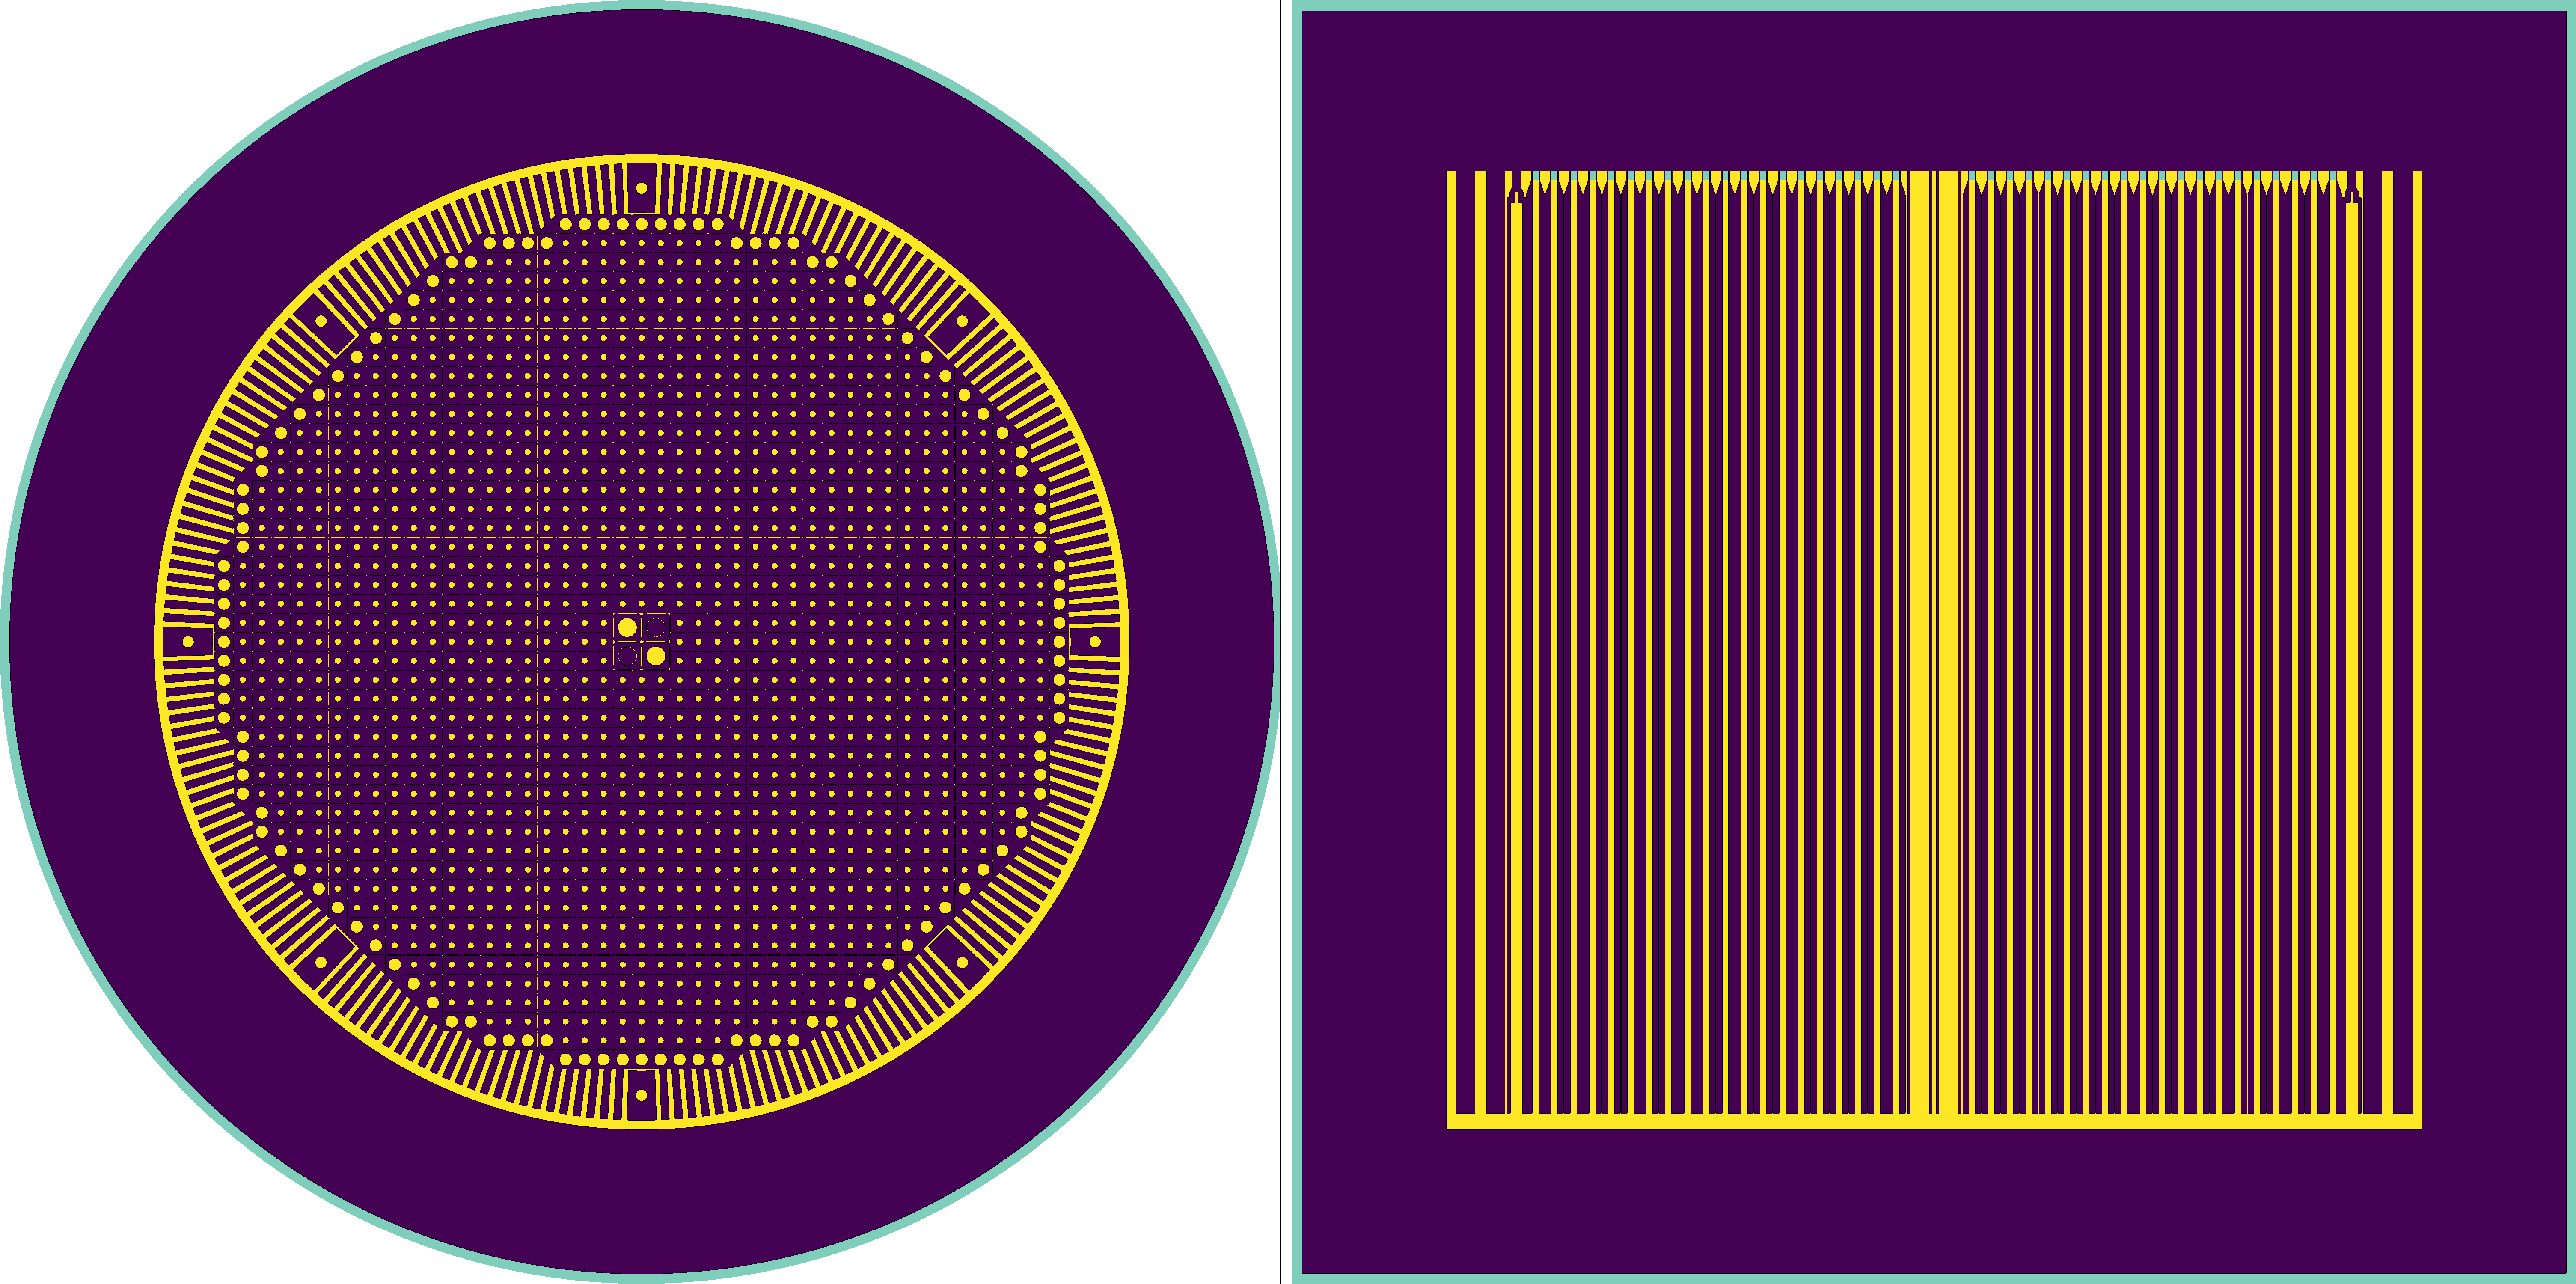
\includegraphics[width=\textwidth]{ch3/view_serpent.png}
	\caption{$XY$ (left) and $XZ$ (right) views of Serpent \gls{MSBR} model 
	(figure reproduced from Rykhlevskii \emph{et al.} 
	\cite{rykhlevskii_modeling_2019}).}
	\label{fig:serpent_plan_view}
\end{figure}

\begin{figure}[t!] % replace 't' with 'b' to \centering
	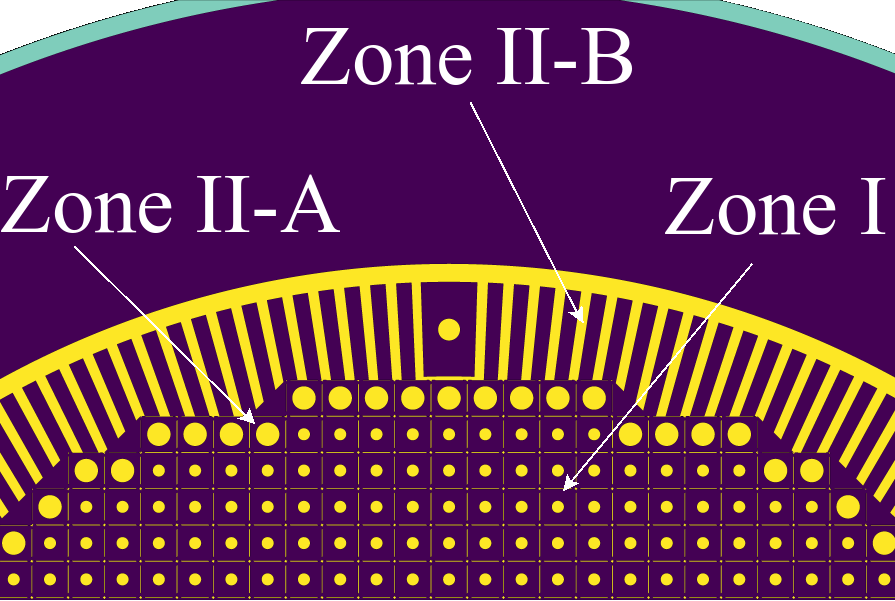
\includegraphics[width=\textwidth]{ch3/ser_zone_II.png}
	\caption{Detailed view of \gls{MSBR} two zone model. 
		Yellow represents fuel salt, purple represents graphite, and aqua 
		represents the reactor vessel. Figure reproduced from Rykhlevskii 
		\emph{et al.} \cite{rykhlevskii_modeling_2019}.}
	\label{fig:serpent_zoneII}
\end{figure}

Since reactor graphite experiences significant dimensional changes due to 
neutron irradiation, the reactor core was designed for periodic replacement. 
Based on the experimental irradiation data from the \gls{MSRE}, the core 
graphite lifetime is about 4 years and the reflector graphite lifetime is 30 
years \cite{robertson_conceptual_1971}.

There are eight symmetric graphite slabs with a width of 15.24 cm in zone II, 
one of which is illustrated in Figure~\ref{fig:serpent_zoneII}. The holes in 
the centers are for the core lifting rods used during the core replacement 
operations. These holes also allow a portion of the fuel salt to flow to the 
top of the vessel for cooling the top head and axial reflector.  
Figure~\ref{fig:serpent_zoneII} also shows the 5.08-cm-wide annular 
space between the removable core graphite in zone II-B and the permanently 
mounted reflector graphite. This annulus consists entirely of fuel salt, 
provides space for moving the core assembly, helps compensate for the 
elliptical dimensions of the reactor vessel, and serves to reduce the damaging 
flux at the surface of the graphite reflector blocks. 

$^{135}$Xe is a strong neutron poison, and some fraction of this gas is 
absorbed by graphite during \gls{MSBR} operation. ORNL calculations show 
that for unsealed commercial graphite with helium permeability 10$^{-5}$ 
cm$^2$/s the calculated poison fraction is less than 2\%  
\cite{robertson_conceptual_1971}.  This parameter can be improved by using 
experimental graphites or by applying sealing technology. The effect of the 
gradual poisoning of the core graphite with xenon is not treated here.

\subsection{Core zone I}
The central region of the core, called zone I, is made up of graphite 
elements, each $10.16$cm$\times$ 10.16cm$\times$396.24cm. Zone I has 4 
channels for control rods: two for graphite rods which both regulate and shim 
during normal operation, and two for backup safety rods consisting of boron 
carbide clad to assure sufficient negative reactivity for emergency situations.

These graphite elements have a mostly rectangular shape with lengthwise ridges 
at each corner that leave space for salt flow elements. Various element sizes 
reduce the peak damage flux and power density in the center of the core to 
prevent local graphite damage.  Figure~\ref{fig:I_element_ref} shows the 
elevation and plan views of graphite elements of zone I 
\cite{robertson_conceptual_1971} and their Serpent model 
\cite{rykhlevskii_full-core_2017}.
\begin{figure}[ht!] % replace 't' with 'b' to \centering
	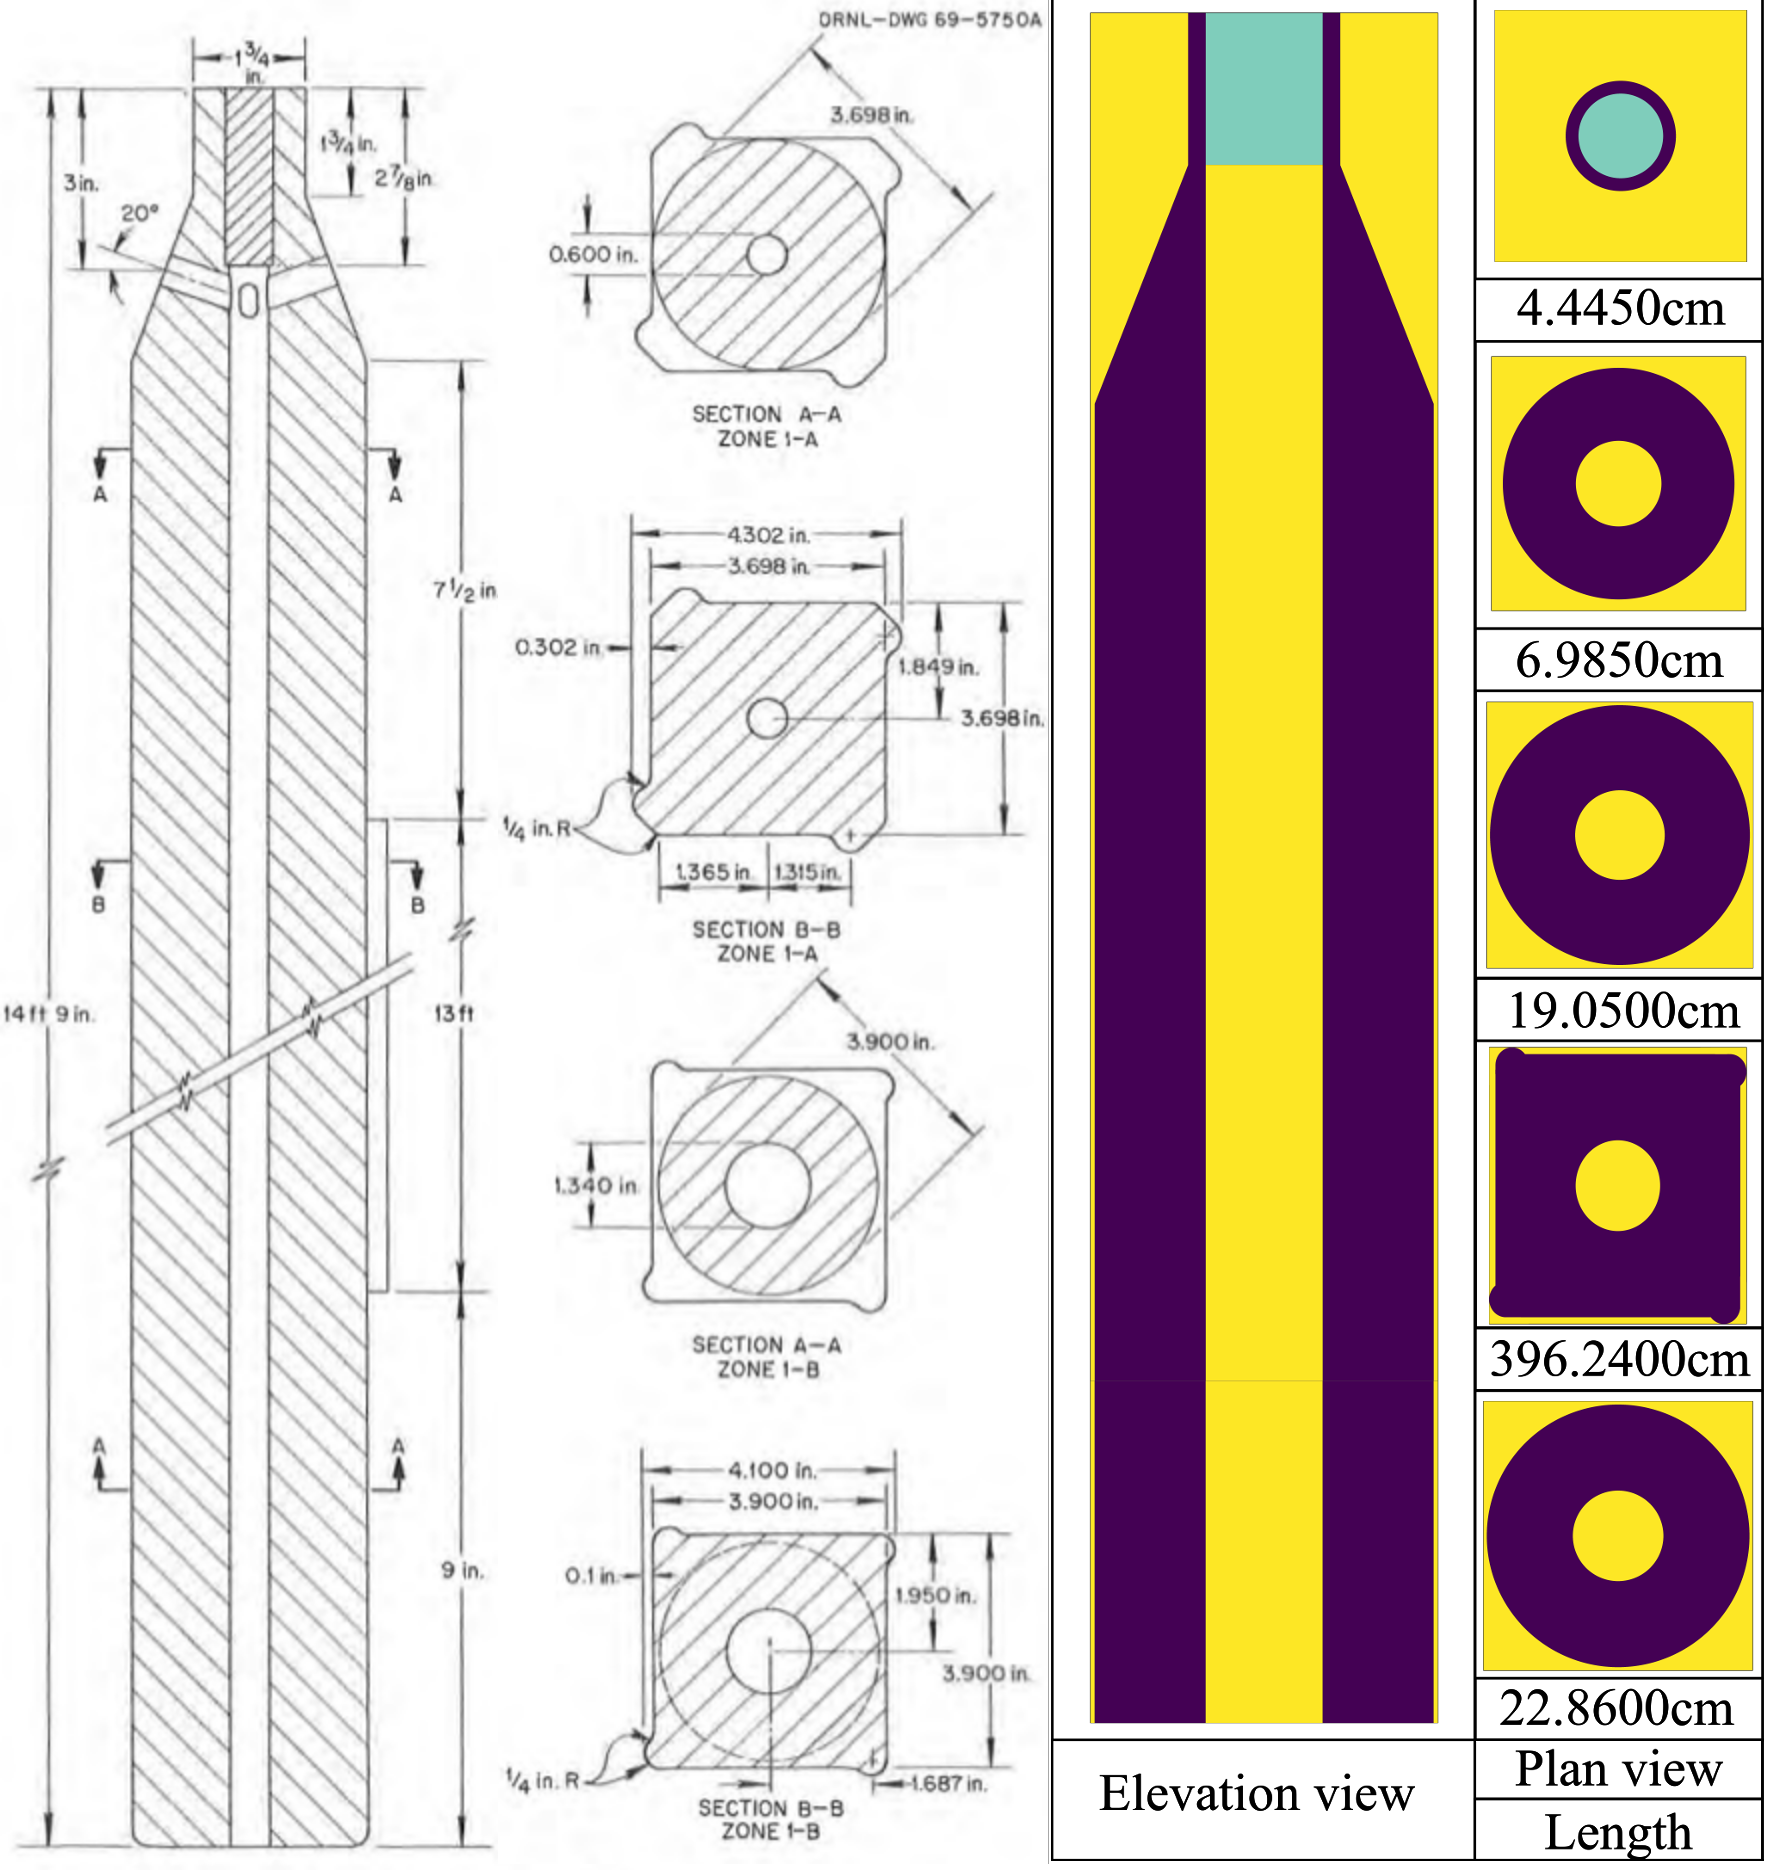
\includegraphics[width=\textwidth]{ch3/zone_I_element_ref.png}
	\caption{Graphite moderator elements for zone I : reference design (left)
		\cite{robertson_conceptual_1971} and Serpent model (right) 
		\cite{rykhlevskii_full-core_2017}.  Yellow 
		represents fuel salt, purple represents graphite, and aqua represents 
		the reactor vessel. Figure reproduced from Rykhlevskii \emph{et al.} 
		\cite{rykhlevskii_modeling_2019}.}
	\label{fig:I_element_ref}
\end{figure}

\subsection{Core zone II}
Zone II, which is undermoderated, surrounds zone I. Combined with the bounding 
radial reflector, zone II serves to diminish neutron leakage. Two kinds of 
elements form this zone: large-diameter fuel channels (zone II-A) and 
radial graphite slats (zone II-B). 

Zone II has 37\% fuel salt by volume and each element has a fuel channel 
diameter of 6.604cm. The graphite elements for zone II-A are prismatic with
elliptical dowels running axially between the prisms. These dowels
isolate the fuel salt flow in zone I from that in zone II.  
Figure~\ref{fig:II_element_ref} shows the shapes and dimensions of these 
graphite elements and their Serpent model. Zone II-B elements are rectangular 
slats spaced far enough apart to provide the 0.37 fuel salt volume fraction. 
The reactor zone II-B graphite 5.08cm-thick slats vary in the radial dimension 
(average width is 26.67cm) as shown in figure~\ref{fig:serpent_zoneII}. Zone 
II serves as a blanket to achieve the best performance: a high breeding ratio 
and a low fissile inventory. The harder neutron energy spectrum in zone II 
enhances the rate of thorium resonance capture relative to the fission rate, 
thus limiting the neutron flux in the outer core zone and reducing the neutron 
leakage \cite{robertson_conceptual_1971}. 

The sophisticated, irregular shapes of the fuel elements challenge an accurate 
representation of zone II-B. The suggested design 
\cite{robertson_conceptual_1971} of zone II-B has 8 irregularly-shaped 
graphite elements as well as dozens of salt channels. These graphite elements 
were simplified into right-circular cylindrical shapes with central channels. 
Figure~\ref{fig:serpent_zoneII} illustrates this core region in the Serpent 
model. The volume of fuel salt in zone II was kept exactly at 37\%, so that 
this simplification did not considerably change the core neutronics. 
Simplyfying the eight edge channels was the only simplification made to the 
\gls{MSBR} geometry in this work. 
\begin{figure}[ht!] % replace 't' with 'b' to \centering
	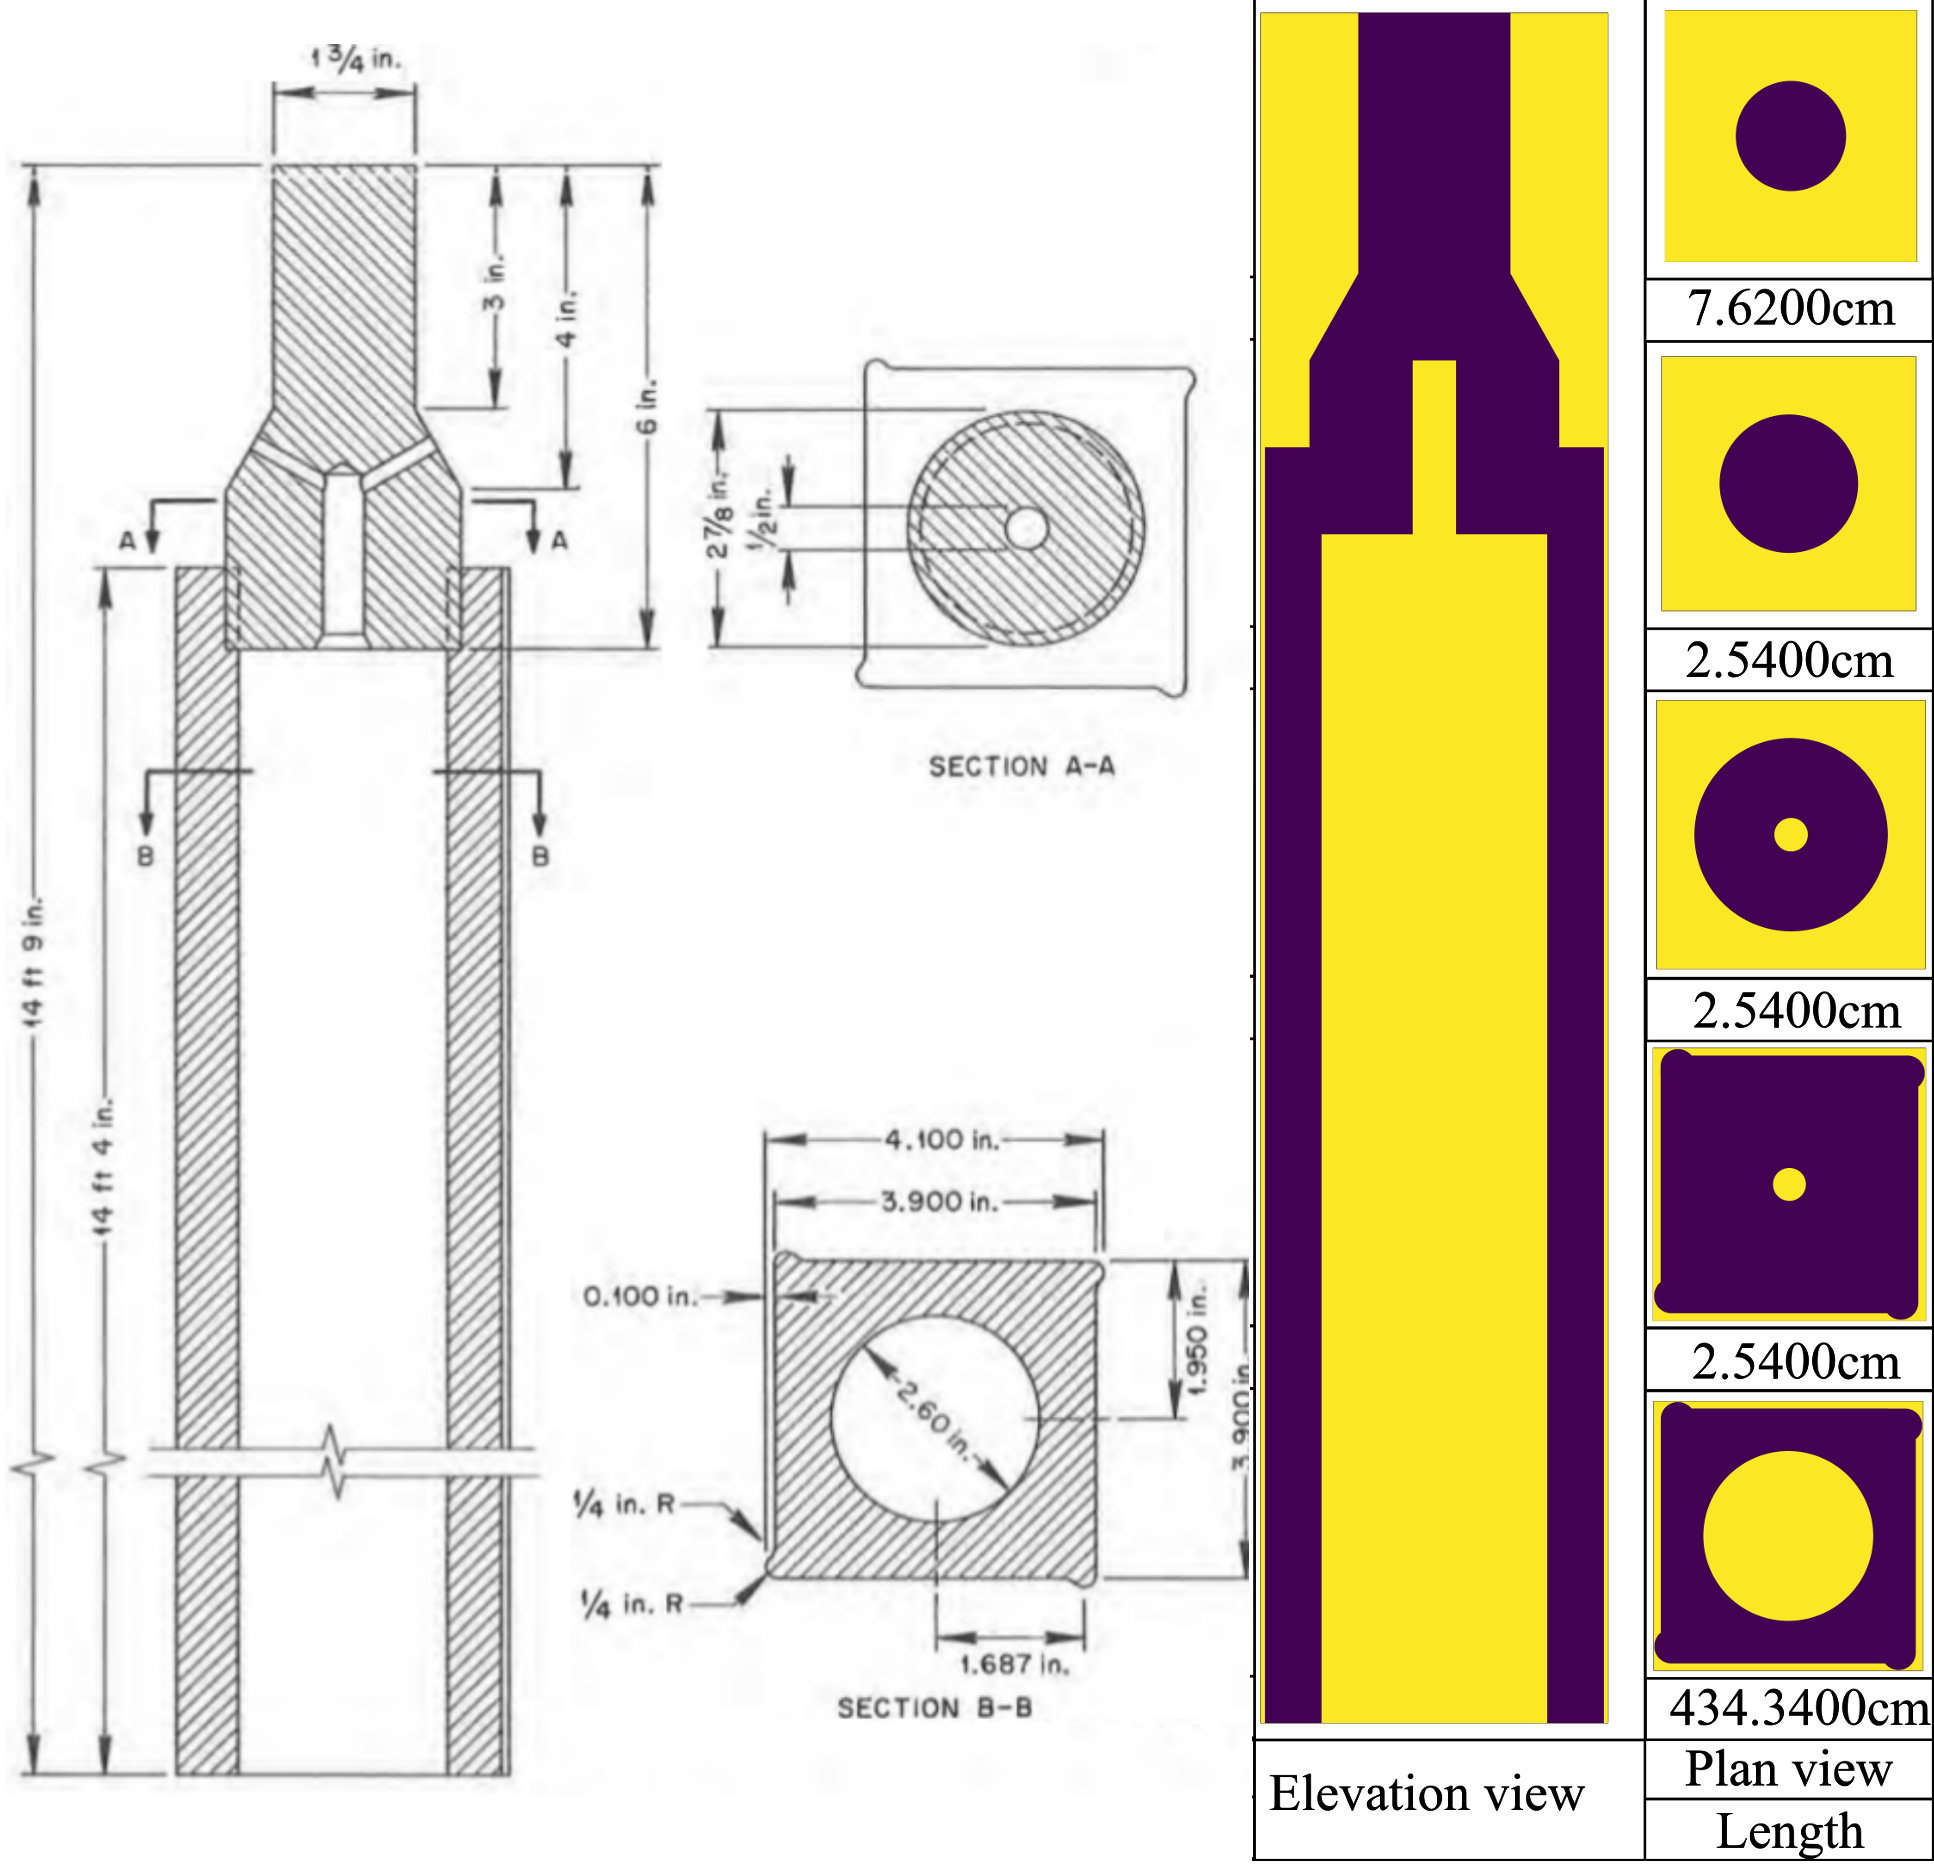
\includegraphics[width=\textwidth]{ch3/zone_II_element_ref.png}
	\caption{Graphite moderator elements for zone II-A: reference design (left)
		\cite{robertson_conceptual_1971} and Serpent model (right) 
		\cite{rykhlevskii_full-core_2017}.  Yellow 
		represents fuel salt, purple represents graphite, and aqua represents 
		the reactor vessel. Figure reproduced from Rykhlevskii \emph{et al.} 
		\cite{rykhlevskii_modeling_2019}.}
	\label{fig:II_element_ref}
\end{figure}

\subsection{Material composition and normalization parameters}
The fuel salt, reactor graphite, and modified Hastelloy-N
are all materials created at \gls{ORNL} specifically for the \gls{MSBR}.
The initial fuel salt used the same density (3.35 g/cm$^3$) and composition 
LiF-BeF$_2$-ThF$_4$-$^{233}$UF$_4$ (71.75-16-12-0.25 mole \%) as the 
\gls{MSBR} design \cite{robertson_conceptual_1971}. The lithium in the molten 
salt fuel is fully enriched to 100\% $^{7}$Li because $^{6}$Li is a very 
strong neutron poison and becomes tritium upon neutron capture. 

The specific temperature was fixed for each material and did not change during 
the reactor operation. The isotopic composition of each material at the 
initial state was described in detail in the MSBR conceptual design study 
\cite{robertson_conceptual_1971} and has been applied to the Serpent model 
without any modification. Table~\ref{tab:msbr_tab} is a summary of the major 
\gls{MSBR} parameters used to inform Serpent model  
\cite{robertson_conceptual_1971}. 
%%%%%%%%%%%%%%%%%%%%%%%%%%%%%%%%%%%%%%%%
\begin{table}[h!]
	\caption{Summary of principal data for \gls{MSBR} 
		\cite{robertson_conceptual_1971}.}
	\begin{tabularx}{\textwidth}{ X  X}
		\hline
		Thermal power           		& 2250 MW$_{th}$		\\
		Electric power             		& 1000 MW$_e$           \\
		Gross thermal efficiency       	& 44.4\%         		\\
		Salt volume fraction in central zone I		& 0.13   	\\
		Salt volume fraction in outer zone II       & 0.37		\\
		Fuel salt inventory (Zone I)                & 8.2 m$^3$	\\
		Fuel salt inventory (Zone II)               & 10.8 m$^3$\\
		Fuel salt inventory (annulus)               & 3.8 m$^3$	\\
		Total fuel salt inventory                   & 48.7 m$^3$\\
		Fissile mass in fuel salt                   & 1303.7 kg	\\
		Fuel salt components   	& LiF-BeF$_2$-ThF$_4$-$^{233}$UF$_4$	\\  
		Fuel salt composition   & 71.75-16-12-0.25 mole\%		\\
		Fuel salt density       & 3.35 g/cm$^3$         		\\ \hline
	\end{tabularx}
	\label{tab:msbr_tab}
\end{table}
%%%%%%%%%%%%%%%%%%%%%%%%%%%%%%%%%%%%%%%%%%%%%%%%

As mentioned in section~\ref{sec:reproc-plant}, the \gls{MSBR} design 
requires online reprocessing to remove neutron gaseous \glspl{FP} (Xe, Kr) and 
noble metals (e.g., Se, Nb, Mo) every 20 seconds.  The $^{232}$Th in the fuel 
absorbs thermal neutrons and produces $^{233}$Pa which then decays into the 
fissile $^{233}$U. Protactinium presents a challenge, since it has a large 
absorption cross section in the thermal energy spectrum. Moreover, $^{233}$Pa 
left in the core would produce $^{234}$Pa and $^{234}$U, neither of which are 
useful as fuel. Accordingly, $^{233}$Pa is continuously removed from the fuel 
salt into a protactinium decay tank to allow $^{233}$Pa to decay to $^{233}$U 
without the corresponding negative neutronic impact. The reactor chemical 
processing system must separate $^{233}$Pa from the molten salt fuel over 3 
days, hold it while $^{233}$Pa decays into $^{233}$U, and return it back to 
the primary loop. This feature allows the reactor to avoid neutron losses to 
protactinium, lowers in-core fission product inventory, and increases the 
efficiency of $^{233}$U breeding.

Table~\ref{tab:reprocessing_list_msbr} summarizes a full list of nuclides and 
their cycle time used for modeling salt treatment and separations 
\cite{robertson_conceptual_1971}. The removal rates vary among chemical 
elements in this reactor concept and dictate the necessary resolution of 
depletion calculations. If the depletion time intervals are very short, an 
enormous number of depletion steps are required to obtain the equilibrium 
composition. On the other hand, if the depletion  calculation time interval is 
too long, the impact of short-lived fission products is not captured. To 
compromise, a 3-day time interval was selected for depletion calculations to 
correlate with the removal interval of $^{233}$Pa, and $^{232}$Th was 
continuously added to maintain the initial mass fraction of $^{232}$Th.
%%%%%%%%%%%%%%%%%%%%%%%%%%%%%%%%%%%%%%%%
\begin{table}[ht!]
	\caption{The cycle times for protactinium and fission 
		products removal from the \gls{MSBR} (reproduced from Robertson 
		\emph{et al.} 
		\cite{robertson_conceptual_1971}).}
	\begin{tabularx}{\textwidth}{x  s  x}
		\hline \textbf{Processing group} & \qquad\qquad\qquad 
		\textbf{Nuclides} & \textbf{Cycle time (at full power)} \\ \hline 
		Rare earths & Y, La, Ce, Pr, Nd, Pm, Sm, 
		Gd & 50 days \\ \qquad & Eu & 500 days \\ Noble metals & Se, 
		Nb, Mo, Tc, Ru, Rh, Pd, Ag, Sb, Te & 20 sec \\
		Seminoble metals & Zr, Cd, In, Sn & 200 days \\
		Gases & Kr, Xe & 20 sec \\ Volatile fluorides & Br, I & 60 days \\
		Discard & Rb, Sr, Cs, Ba & 3435 days \\ 
		%Salt discard & Th, Li, Be, F & 3435 days \\ 
		Protactinium & $^{233}$Pa & 3 days \\ Higher 
		nuclides & $^{237}$Np, $^{242}$Pu & 16 years \\  \hline
	\end{tabularx}
	\label{tab:reprocessing_list_msbr}
\end{table}
%%%%%%%%%%%%%%%%%%%%%%%%%%%%%%%%%%%%%%%%%

\section{Fuel salt isotopic composition dynamics and equilibrium search}
The SaltProc online reprocessing simulation package is demonstrated in four 
applications: (1) analyzing the \gls{MSBR} neutronics and fuel cycle to find 
the equilibrium core composition and fuel salt depletion, (2) studying 
operational and safety parameters evolution during \gls{MSBR} operation, (3) 
demonstrating that in a single-fluid two-region \gls{MSBR} conceptual design 
the undermoderated outer core zone II works as a virtual ``blanket'', reduces 
neutron leakage and improves breeding ratio due to neutron energy spectral 
shift, and (4) determining the effect of fission product removal on the core 
neutronics.

The neutron population per cycle and the number of active/inactive cycles were 
chosen to obtain balance between reasonable uncertainty for a transport 
problem ($\leq$ 15 pcm\footnote{ 1 pcm = 10$^{-5}\Delta k_{eff}/k_{eff}$} for 
effective multiplication factor) and computational time. The \gls{MSBR} 
depletion and safety parameter computations were performed on 64 Blue Waters 
XK7 nodes (two AMD 6276 Interlagos CPU per node, 16 floating-point Bulldozer 
core units per node or 32 ``integer'' cores per node, nominal clock speed is 
2.45 GHz). The total computational time for calculating the equilibrium 
composition was approximately 9,900 node-hours (18 core-years.)

\subsection{Effective multiplication factor dynamics}
Figures~\ref{fig:keff}, \ref{fig:keff_zoomed} show the effective 
multiplication factors obtained using SaltProc and Serpent. The effective 
multiplication factors were calculated after removing fission products listed 
in  Table~\ref{tab:reprocessing_list_msbr} and adding the fertile material at 
the end of cycle time (3 days). The effective multiplication factor fluctuates 
significantly as a result of the batch-wise nature of this online reprocessing 
strategy. 
\begin{figure}[ht!] 
	\centering
	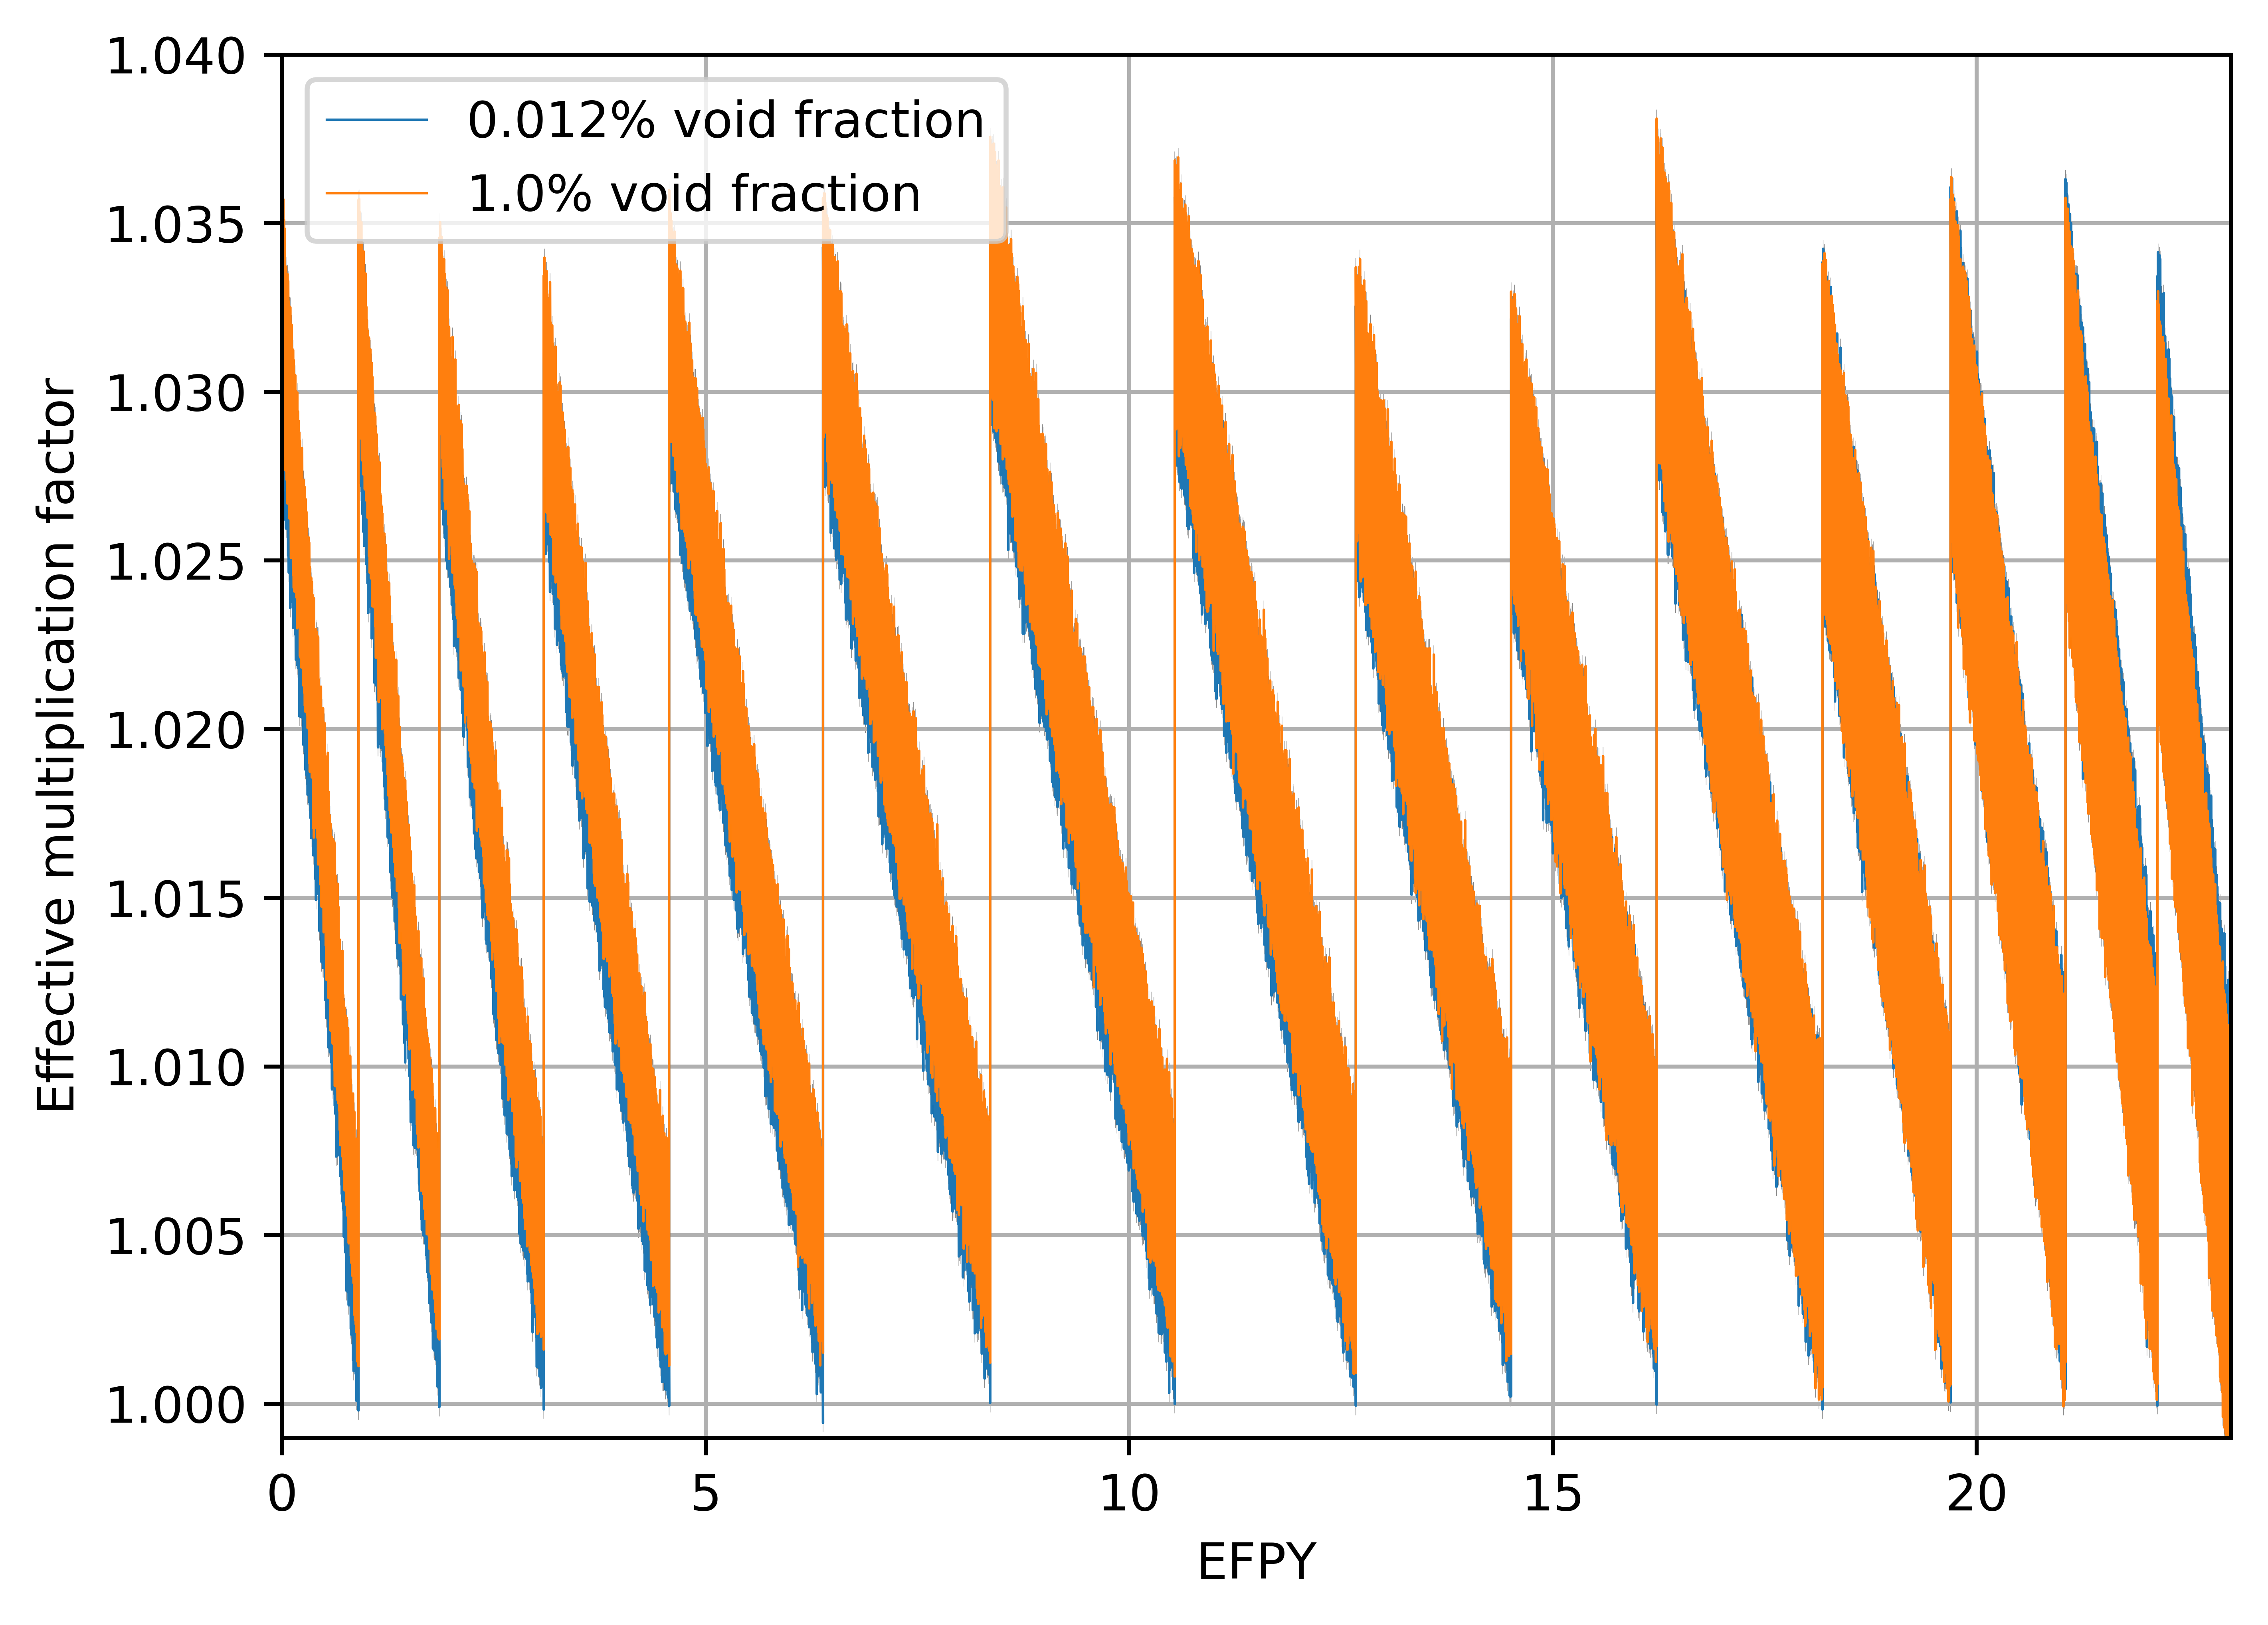
\includegraphics[width=\textwidth]{ch3/keff.png}
	\caption{Effective multiplication factor dynamics for full-core \gls{MSBR} 
		model over a 60-year reactor operation lifetime. Figure reproduced 
		from Rykhlevskii \emph{et al.} \cite{rykhlevskii_modeling_2019}.}
	\label{fig:keff}
\end{figure}
\begin{figure}[ht!] 
	\centering
	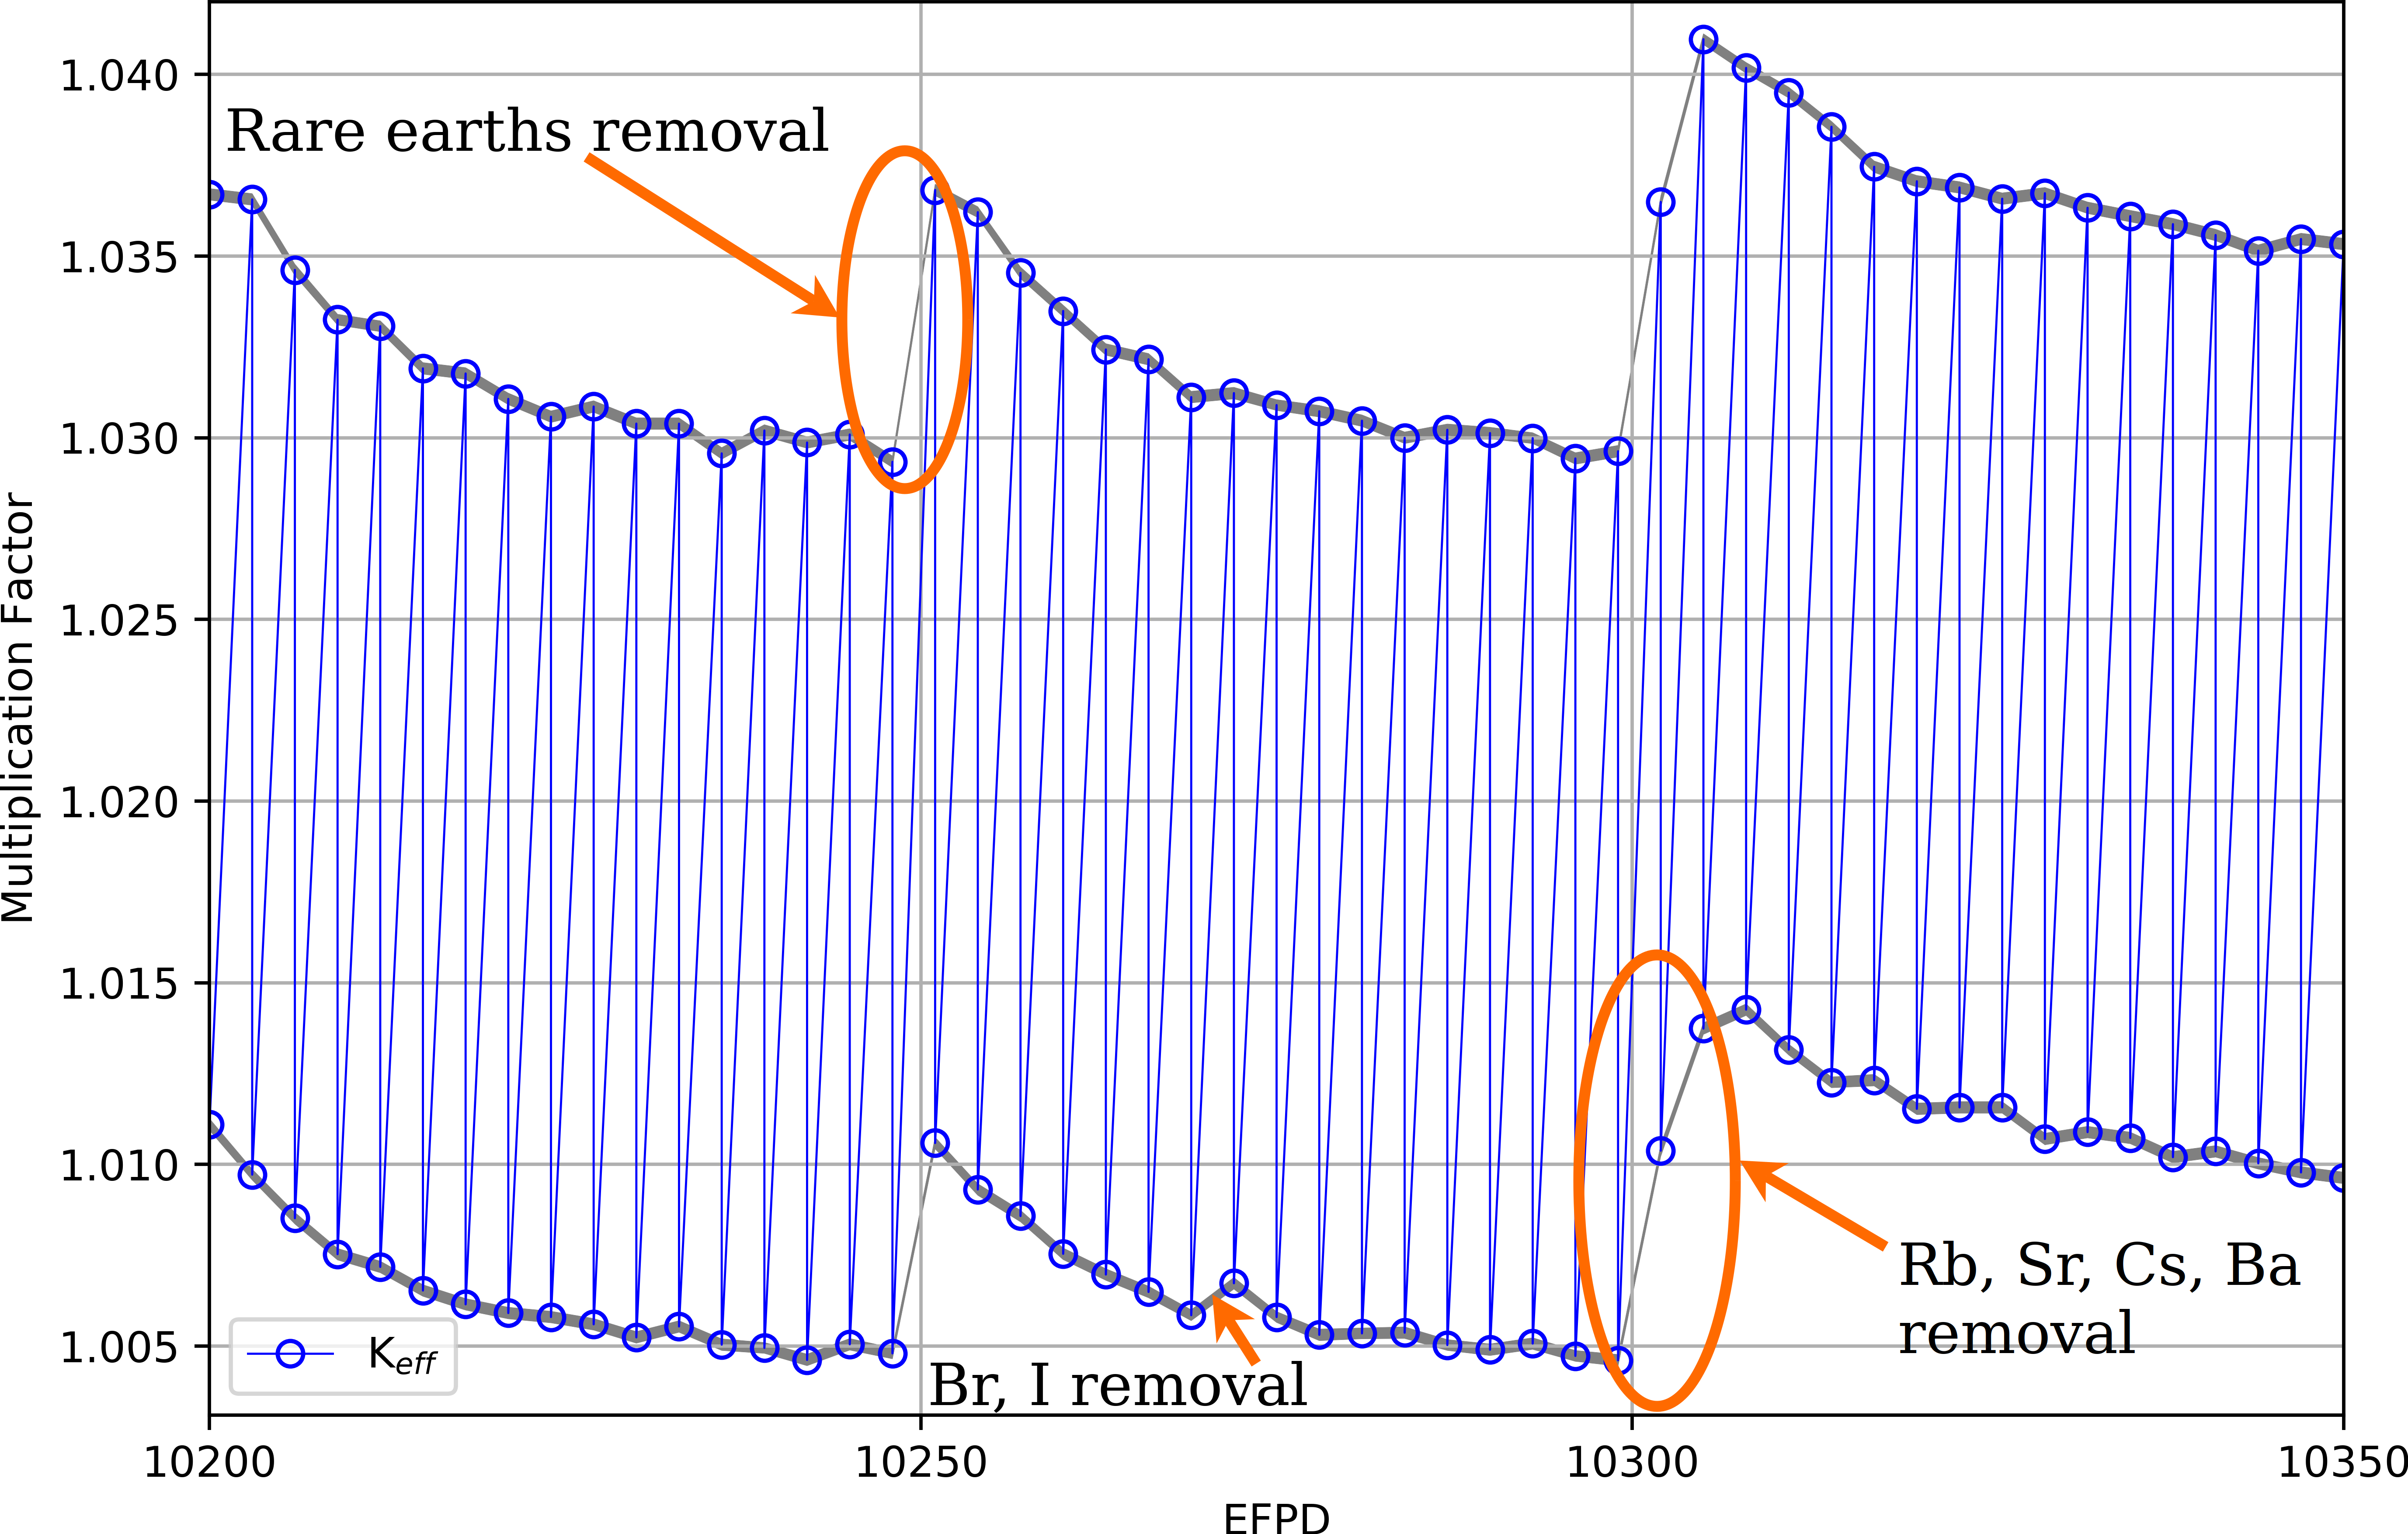
\includegraphics[width=\textwidth]{ch3/keff_zoomed.png}
	\caption{Zoomed effective multiplication factor for 150-EFPD time 
	interval. Figure reproduced from Rykhlevskii \emph{et al.}  
	\cite{rykhlevskii_modeling_2019}.}
	\label{fig:keff_zoomed}
\end{figure}

First, Serpent calculates the effective multiplication factor for the  
beginning of the cycle (there is fresh fuel composition at the first step). 
Next, it computes the new fuel salt composition at the end of a 3-day 
depletion. The corresponding effective multiplication factor is much smaller 
than the previous one. Finally, SERPENT calculates $k_{eff}$ for the depleted 
composition after applying feeds and removals. The $K_{eff}$ increases 
accordingly since major reactor poisons (e.g. Xe, Kr) are removed, while fresh 
fissile material ($^{233}$U) from the protactinium decay tank is added.  

Additionally, the presence of rubidium, strontium, cesium, and barium in the 
core are disadvantageous to reactor physics. Overall, the effective 
multiplication factor gradually decreases from 1.075 to $\approx$1.02 at 
equilibrium after approximately 6 years of irradiation. 

In fact, SaltProc v0.1 fully removes all of these elements every 3435 days 
(not a small mass fraction every 3 days) which causes the multiplication 
factor to jump by approximately 450 pcm, and limits using the batch approach 
for online reprocessing simulations. In SaltProc v1.0 this drawback has been  
eliminated by removing fraction of element at each depletion step with longer 
residence times (seminoble metals, volatile fluorides, Rb, Sr, Cs, Ba, Eu).  
Results with taking into account this approach wiil be presented for the 
\gls{TAP} \gls{MSR} in chapter 4.

\section{Operational and safety parameters evolution}

\section{Benefits of fission product removal}

\section{Concluding remarks}